\section*{Task 2}

\subsection*{Task statement}
Synchronize your 6 joints to start and end motion at the same time.

\subsection*{Solution}

To synchronize the joints, we should find maximum $t_b$ and $t_{na}$ (for triangular ones I set $t_{na} = 0$), then $t_{b_{max}}, t_{na_{max}}$ are the maximum time spend on blend phase and non-acceleration phase.

Then we define new constraints on velocity and acceleration for each joint:

$$\dot q_i = \frac{\Delta q_i}{t_{b_{max}} + t_{na_{max}}}$$
$$\ddot q_i = \frac{\dot q_i}{t_{b_{max}}}$$

Then we just recalculate trajectories with these new constraints

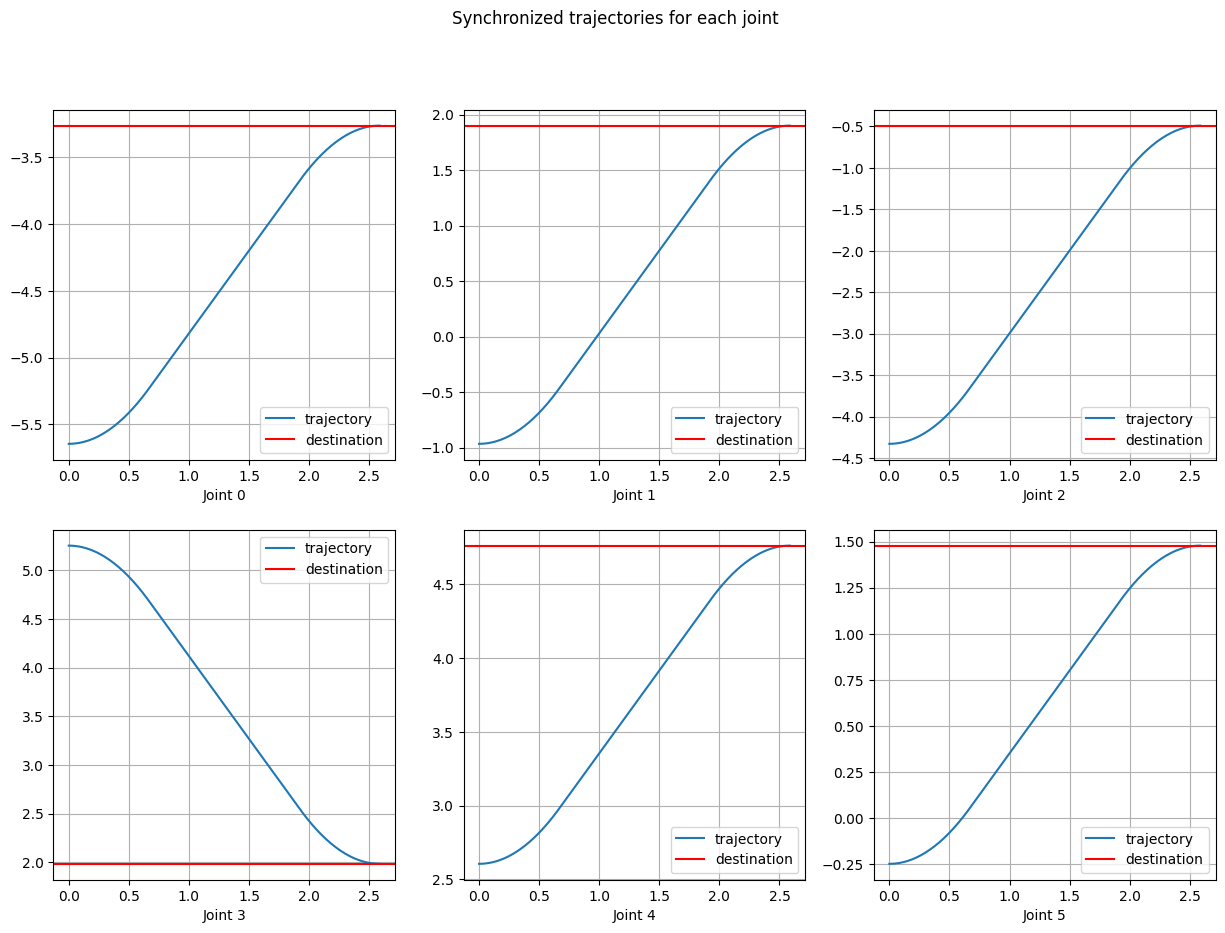
\includegraphics[width=\linewidth]{images/trajectory_synchronized.png}